\documentclass[11pt,a4paper,oneside]{article}\usepackage[]{graphicx}\usepackage[]{color}
%% maxwidth is the original width if it is less than linewidth
%% otherwise use linewidth (to make sure the graphics do not exceed the margin)
\makeatletter
\def\maxwidth{ %
  \ifdim\Gin@nat@width>\linewidth
    \linewidth
  \else
    \Gin@nat@width
  \fi
}
\makeatother

\definecolor{fgcolor}{rgb}{0.345, 0.345, 0.345}
\newcommand{\hlnum}[1]{\textcolor[rgb]{0.686,0.059,0.569}{#1}}%
\newcommand{\hlstr}[1]{\textcolor[rgb]{0.192,0.494,0.8}{#1}}%
\newcommand{\hlcom}[1]{\textcolor[rgb]{0.678,0.584,0.686}{\textit{#1}}}%
\newcommand{\hlopt}[1]{\textcolor[rgb]{0,0,0}{#1}}%
\newcommand{\hlstd}[1]{\textcolor[rgb]{0.345,0.345,0.345}{#1}}%
\newcommand{\hlkwa}[1]{\textcolor[rgb]{0.161,0.373,0.58}{\textbf{#1}}}%
\newcommand{\hlkwb}[1]{\textcolor[rgb]{0.69,0.353,0.396}{#1}}%
\newcommand{\hlkwc}[1]{\textcolor[rgb]{0.333,0.667,0.333}{#1}}%
\newcommand{\hlkwd}[1]{\textcolor[rgb]{0.737,0.353,0.396}{\textbf{#1}}}%

\usepackage{framed}
\makeatletter
\newenvironment{kframe}{%
 \def\at@end@of@kframe{}%
 \ifinner\ifhmode%
  \def\at@end@of@kframe{\end{minipage}}%
  \begin{minipage}{\columnwidth}%
 \fi\fi%
 \def\FrameCommand##1{\hskip\@totalleftmargin \hskip-\fboxsep
 \colorbox{shadecolor}{##1}\hskip-\fboxsep
     % There is no \\@totalrightmargin, so:
     \hskip-\linewidth \hskip-\@totalleftmargin \hskip\columnwidth}%
 \MakeFramed {\advance\hsize-\width
   \@totalleftmargin\z@ \linewidth\hsize
   \@setminipage}}%
 {\par\unskip\endMakeFramed%
 \at@end@of@kframe}
\makeatother

\definecolor{shadecolor}{rgb}{.97, .97, .97}
\definecolor{messagecolor}{rgb}{0, 0, 0}
\definecolor{warningcolor}{rgb}{1, 0, 1}
\definecolor{errorcolor}{rgb}{1, 0, 0}
\newenvironment{knitrout}{}{} % an empty environment to be redefined in TeX

\usepackage{alltt}
\usepackage{amsmath,amsthm,amsfonts,amssymb}
\usepackage{pst-eucl,pstricks,pstricks-add}
%\usepackage[utf8]{inputenc}
%\usepackage[latin1]{inputenc}
\usepackage[spanish,activeacute]{babel}
\usepackage[a4paper,margin=2.5cm]{geometry}
\usepackage{times}
\usepackage[T1]{fontenc}
\usepackage{titlesec}
\usepackage{color}
\usepackage{url}
\usepackage{float}
\usepackage{cite}
\usepackage{graphicx}
\usepackage{multicol}
\usepackage{float}
\usepackage{lmodern}
\parindent=0mm
\IfFileExists{upquote.sty}{\usepackage{upquote}}{}
\begin{document}

\thispagestyle{empty}
{\sf
{\Large \scshape Escuela Polit\'{e}cnica Nacional} \hfill {\scshape 18 de Diciembre 2015}\\[3mm] 
{\scshape C\'{a}lculo en una variable \hfill Prueba $\#7$}\\[7mm]
{\scshape Nombre:} \rule{0.6\textwidth}{0.5pt}\qquad {\scshape Nro. lista:} \rule{0.1\textwidth}{0.5pt}\\
}




\begin{enumerate}
      \item Calcule el siguiente límite: $\displaystyle \lim_{n\to \infty} \frac{n + 2n + 3n + \ldots + (n-1)n + n^2}{n^2 + (n-1)^2 + \ldots + 3^2 + 2^2 + 1^2}$\\[5cm]
      
      \item Use la prueba de la primera y segunda derivada para encontrar los extremos relativos, extremos absolutos, puntos de inflexión e intervalos de concavidad y convexidad de la función $f(x)=2x^4+x^3-14x^2+5x+6$, en el intervalo $x\in [ -\frac{7}{2},3]$. Grafique.\\[13cm]
      
      \item Un cuadrado está inscrito en un círculo de radio $r$, como se muestra en la figura. ?`A qué razón cambia el área del cuadrado en el instante en que el radio del círculo mide 2 pulg y crece a razón de 4 pulg/min?.
      
      \begin{figure}[H]
      \centering
      \begin{pspicture}[showgrid=false](2,2)
      \pscircle[linecolor=red](1,1){1.15}
      \psframe[linecolor=blue](0.2,0.2)(1.8,1.8)
      \psline{->}(1,1)(1,2.15)
      \rput(1.2,1.5){$r$}
      \end{pspicture}
      \end{figure}
      
      \vspace{6cm}
      
      \item Se producirá una caja, abierta por la parte superior, de una pieza rectangular de cartón que mide 50 cm de largo por 40 cm de ancho. La caja puede cerrarse al cortar un cuadrado en cada esquina, al cortar sobre las líneas sólidas interiores y doblar luego el cartón por las líneas discontinuas. Exprese el volumen de la caja como una función de la variable indicada x. Encuentre las dimensiones de la caja con que se obtiene el volumen máximo. ?`Cuál es el volumen máximo?
      
      \begin{figure}[H]
      \centering
      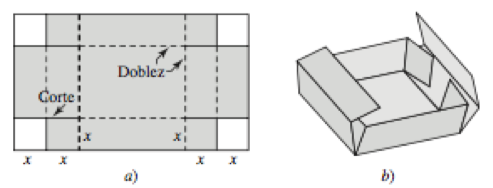
\includegraphics[scale=0.45]{fig02.png}
      \end{figure}
      
      \vspace{8cm}
      
      \item Determinar las dimensiones del cono circular recto de máximo volumen que puede inscribirse en una esfera de radio R.
      
      \begin{figure}[H]
      \centering
      \begin{pspicture}[showgrid=false](4,3)
      \pscircle[linecolor=red](2,1.5){1.5}
      \psline[linecolor=blue](0.7,0.7)(3.3,0.7)(2,3)(0.7,0.7)
      \psline[linewidth=1.5pt]{->}(2,1.5)(2,0)
      \rput(2.2,0.5){\small R}
      \rput(2,3.3){\scriptsize Corte transversal}
      \end{pspicture}
      \end{figure}
      
      
\end{enumerate}

\end{document}
